\documentclass[aspectratio=169,xcolor=dvipsnames]{beamer}
\usetheme{Madrid}
\usecolortheme{seahorse}
\usepackage{amsmath,amssymb,booktabs,hyperref,listings,tikz}
\lstset{
  language=Python,
  basicstyle=\small\ttfamily,
  keywordstyle=\color{blue}\bfseries,
  commentstyle=\color{OliveGreen},
  stringstyle=\color{red},
  frame=single,
  breaklines=true
}

\title[Algorithms -- Week 5]{\textbf{Design and Analysis of Algorithms}\\
\large Week 5: Greedy Algorithms I -- Classic Paradigm \& Problems}
\subtitle{TOAE209/TOAH209 -- Foreign Trade University}
\author{Department of Technology \& Data Science}
\date{Semester 2024--2025}

\AtBeginSection[]{
  \begin{frame}<beamer>{Outline}
    \tableofcontents[currentsection]
  \end{frame}
}

\begin{document}

\begin{frame}
  \titlepage
\end{frame}

\begin{frame}{Outline}
  \tableofcontents
\end{frame}

% ==========================================
\section{The Greedy Paradigm}
% ==========================================

\begin{frame}{What is the Greedy Paradigm?}
  \begin{itemize}
    \item At each step, choose the option that looks **best in the short term**.
    \item Make a locally optimal choice in the hope that it leads to a globally optimal solution.
    \item Unlike Dynamic Programming, once a choice is made, it is **never reconsidered** (no backtracking).
  \end{itemize}
  \begin{block}{Greedy Invariants}
    Usually characterized by:
    \begin{enumerate}
      \item **Greedy choice property:** A global optimum can be reached by making local choices.
      \item **Optimal substructure:** An optimal solution contains optimal solutions to subproblems.
    \end{enumerate}
  \end{block}
\end{frame}

\begin{frame}{Greedy vs Dynamic Programming}
  \begin{center}
  \begin{tabular}{lll}
    \toprule
    \textbf{Dimension} & \textbf{Greedy Paradigm} & \textbf{Dynamic Programming} \\
    \midrule
    Choice & Local choice at each step & Explores all subproblems \\
    Backtracking & Never backs up & Evaluates all overlapping states \\
    Proof of Correctness & Always required (often hard) & Checked via recursive induction \\
    Efficiency & Usually $\mathcal{O}(n \log n)$ or $\mathcal{O}(n)$ & $\mathcal{O}(n^2)$ or higher \\
    \bottomrule
  \end{tabular}
  \end{center}
  \begin{alertblock}{Warning}
    Greedy algorithms are easy to design, but **very hard to prove correct**. Most intuitive greedy heuristics are actually incorrect!
  \end{alertblock}
\end{frame}

% ==========================================
\section{Coin Changing}
% ==========================================

\begin{frame}{Coin Changing Problem}
  \begin{block}{Problem Statement}
    Given an amount $A$ and a set of coin denominations $C = \{c_1, c_2, \ldots, c_d\}$, select the minimum number of coins that sum exactly to $A$.
  \end{block}
  \begin{itemize}
    \item **Greedy Heuristic:** Choose the largest denomination coin $c \le A$, add it to the solution, and repeat for $A - c$.
    \item **Example (US System: $\{25, 10, 5, 1\}$):** For $A = 41$:
      \begin{itemize}
        \item Select $25$ (remaining: $16$)
        \item Select $10$ (remaining: $6$)
        \item Select $5$ (remaining: $1$)
        \item Select $1$ (remaining: $0$)
        \item Total coins: 4 ($25 + 10 + 5 + 1$) -- **Optimal!**
      \end{itemize}
  \end{itemize}
\end{frame}

\begin{frame}{Coin Changing: The Limits of Greedy}
  Does the greedy heuristic work for *every* coin system?
  \begin{alertblock}{No! Counter-example}
    Suppose $C = \{4, 3, 1\}$ and we want to change $A = 6$.
    \begin{itemize}
      \item **Greedy Selection:**
        \begin{itemize}
          \item Select $4$ (remaining: $2$)
          \item Select $1$ (remaining: $1$)
          \item Select $1$ (remaining: $0$)
          \item Total: 3 coins ($4 + 1 + 1$)
        \end{itemize}
      \item **Optimal Selection:**
        \begin{itemize}
          \item Select $3$ and $3$
          \item Total: 2 coins ($3 + 3$)
        \end{itemize}
    \end{itemize}
    Greedy is **sub-optimal** here! General coin changing requires Dynamic Programming.
  \end{alertblock}
\end{frame}

% ==========================================
\section{Interval Scheduling}
% ==========================================

\begin{frame}{Interval Scheduling Problem}
  \begin{block}{Problem Statement}
    Given a set of intervals $J = \{1, 2, \ldots, n\}$ where each interval $i$ has a start time $s_i$ and a finish time $f_i$. Find the **maximum size subset** of mutually compatible (non-overlapping) intervals.
  \end{block}
  \begin{center}
  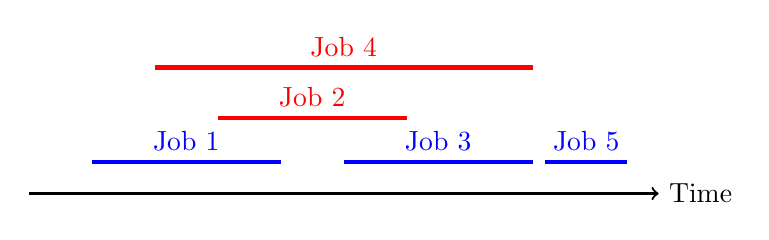
\begin{tikzpicture}[scale=0.8]
    \draw[thick, ->] (0,0) -- (10,0) node[right] {Time};
    \draw[blue, ultra thick] (1,0.5) -- (4,0.5) node[midway, above] {Job 1};
    \draw[red, ultra thick] (3,1.2) -- (6,1.2) node[midway, above] {Job 2};
    \draw[blue, ultra thick] (5,0.5) -- (8,0.5) node[midway, above] {Job 3};
    \draw[red, ultra thick] (2,2) -- (8,2) node[midway, above] {Job 4};
    \draw[blue, ultra thick] (8.2,0.5) -- (9.5,0.5) node[midway, above] {Job 5};
  \end{tikzpicture}
  \end{center}
\end{frame}

\begin{frame}{Interval Scheduling: Heuristics}
  Which greedy sorting strategy is optimal?
  \begin{itemize}
    \item **Strategy 1: Earliest Start Time First** -- Counterexample: one long interval covering the whole timeline prevents all others.
    \item **Strategy 2: Shortest Interval First** -- Counterexample: one short interval overlapping with two long compatible ones.
    \item **Strategy 3: Fewest Conflicts First** -- Counterexample: complicated overlapping clusters.
    \item **Strategy 4: Earliest Finish Time First (EFT)** -- **Optimal!**
  \end{itemize}
  \begin{exampleblock}{EFT Rule}
    Sort by finish time $f_i$ ascending. Select the first interval, then select the next compatible interval, and repeat.
  \end{exampleblock}
\end{frame}

\begin{frame}[fragile]{Interval Scheduling Pseudocode}
  \begin{lstlisting}[language=Python]
def interval_scheduling(intervals):
    # Sort intervals by finish time
    sorted_ints = sorted(enumerate(intervals), key=lambda x: x[1][1])
    selected = []
    last_end = -float('inf')
    for idx, (start, end) in sorted_ints:
        if start >= last_end:
            selected.append(idx)
            last_end = end
    return selected
  \end{lstlisting}
  \begin{block}{Complexity}
    * **Time:** $\mathcal{O}(n \log n)$ due to sorting.
    * **Space:** $\mathcal{O}(n)$ to store indices and sorted list.
  \end{block}
\end{frame}

\begin{frame}{Proof of Optimality: Greedy Stays Ahead}
  Let $A = \{i_1, i_2, \ldots, i_k\}$ be the greedy selection, and $O = \{j_1, j_2, \ldots, j_m\}$ be an optimal selection.
  \begin{block}{Theorem}
    Greedy is optimal, i.e., $k = m$.
  \end{block}
  \begin{proof}
    We prove by induction that for all $r \le k$:
    $$f(i_r) \le f(j_r)$$
    * **Base case ($r=1$):** Greedy picks the interval with earliest finish time overall, so $f(i_1) \le f(j_1)$ holds.
    * **Inductive step:** Assume $f(i_{r-1}) \le f(j_{r-1})$. Since $O$ is compatible, $s(j_r) \ge f(j_{r-1}) \ge f(i_{r-1})$. Thus, $j_r$ is in the set of candidate intervals available to greedy. Since greedy selects the available interval with earliest finish time, $f(i_r) \le f(j_r)$.
    By induction, this holds. If $m > k$, optimal could select $j_{k+1}$, but $s(j_{k+1}) \ge f(j_k) \ge f(i_k)$, meaning greedy would have picked at least one more interval. Contradiction!
  \end{proof}
\end{frame}

% ==========================================
\section{Interval Partitioning}
% ==========================================

\begin{frame}{Interval Partitioning Problem}
  \begin{block}{Problem Statement}
    Given $n$ intervals representing lectures, schedule all of them in the **minimum number of classrooms** such that no two overlapping lectures share a classroom.
  \end{block}
  \begin{center}
  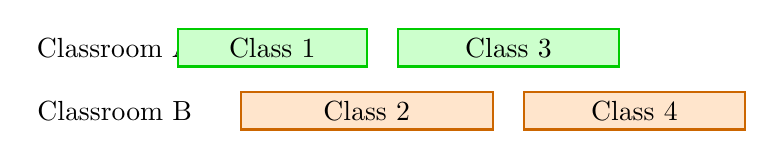
\begin{tikzpicture}[scale=0.8]
    \node at (-1, 1.5) {Classroom A};
    \draw[fill=green!20, draw=green!80!black, thick] (0, 1.2) rectangle (3, 1.8) node[midway] {Class 1};
    \draw[fill=green!20, draw=green!80!black, thick] (3.5, 1.2) rectangle (7, 1.8) node[midway] {Class 3};

    \node at (-1, 0.5) {Classroom B};
    \draw[fill=orange!20, draw=orange!80!black, thick] (1, 0.2) rectangle (5, 0.8) node[midway] {Class 2};
    \draw[fill=orange!20, draw=orange!80!black, thick] (5.5, 0.2) rectangle (9, 0.8) node[midway] {Class 4};
  \end{tikzpicture}
  \end{center}
\end{frame}

\begin{frame}{Interval Partitioning: Lower Bound via Depth}
  \begin{definition}{Depth}
    The **depth** of a set of intervals is the maximum number of intervals that overlap at any single point in time.
  \end{definition}
  \begin{center}
  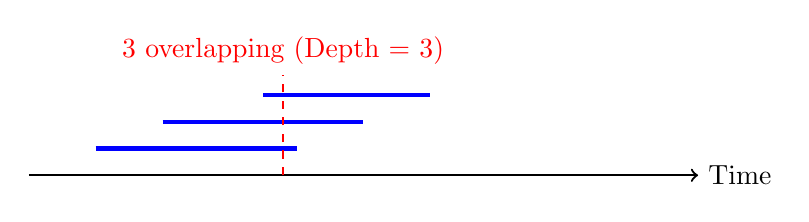
\begin{tikzpicture}[scale=0.85]
    \draw[thick, ->] (0,0) -- (10,0) node[right] {Time};
    \draw[blue, ultra thick] (1,0.4) -- (4,0.4);
    \draw[blue, ultra thick] (2,0.8) -- (5,0.8);
    \draw[blue, ultra thick] (3.5,1.2) -- (6,1.2);
    \draw[dashed, red, thick] (3.8, 0) -- (3.8, 1.5) node[above] {3 overlapping (Depth = 3)};
  \end{tikzpicture}
  \end{center}
  \begin{block}{Lower Bound}
    Since all intervals overlapping at time $t$ must be assigned to different rooms, the number of classrooms needed is **at least** the depth $d$.
  \end{block}
\end{frame}

\begin{frame}{Interval Partitioning: Greedy Strategy}
  \begin{exampleblock}{Greedy Algorithm}
    1. Sort intervals by **start time** $s_i$ ascending.
    2. Go through each interval:
       * If an existing classroom is free, assign the interval to it.
       * If all active classrooms are busy, open a **new classroom**.
  \end{exampleblock}
  \begin{block}{Implementation Hint}
    Store classrooms in a **Min-Heap**, keyed by the finish time of the last lecture assigned to them.
    * Extract min tells you if a classroom is free.
    * Heap size at the end represents the number of rooms needed.
    * **Time Complexity:** $\mathcal{O}(n \log n)$, **Space Complexity:** $\mathcal{O}(n)$.
  \end{block}
\end{frame}

\begin{frame}{Interval Partitioning: Proof of Optimality}
  \begin{proof}
    Let $d$ be the maximum depth of the interval set. We show that greedy uses exactly $d$ classrooms.
    * Suppose greedy allocates classroom $k$. This occurs because when scheduling some interval $i$, all $k-1$ active classrooms are busy.
    * This means at the start time $s_i$, there are $k-1$ other intervals currently running.
    * Including interval $i$, there are $k$ intervals overlapping at time $s_i$.
    * Thus, the depth at $s_i$ is at least $k$.
    * Since max depth is $d$, we must have $k \le d$.
    * Therefore, the number of classrooms allocated by greedy is at most $d$.
    * Since $d$ is a mathematical lower bound, greedy uses **exactly** $d$ classrooms, which is optimal!
  \end{proof}
\end{frame}

% ==========================================
\section{Scheduling to Minimize Lateness}
% ==========================================

\begin{frame}{Scheduling to Minimize Lateness}
  \begin{block}{Problem Statement}
    We have a single machine and $n$ jobs. Each job $i$ has a processing time $t_i$ and a deadline $d_i$.
    If we start at time 0, and job $i$ finishes at time $f_i$, its lateness is:
    $$L_i = \max(0, f_i - d_i)$$
    Find a schedule to **minimize the maximum lateness** $L = \max_i L_i$.
  \end{block}
  \begin{itemize}
    \item **Heuristic 1:** Shortest processing time first -- Counterexample: ignores deadlines.
    \item **Heuristic 2:** Smallest slack time first ($d_i - t_i$) -- Counterexample: breaks down easily.
    \item **Heuristic 3: Earliest Deadline First (EDF)** -- Sort by deadline $d_i$ ascending. **Optimal!**
  \end{itemize}
\end{frame}

\begin{frame}{Minimize Lateness: Proof of Optimality}
  We prove EDF is optimal using an **exchange argument**.
  \begin{definition}{Inversion}
    An **inversion** in a schedule is a pair of jobs $i$ and $j$ such that job $i$ is scheduled before job $j$, but job $j$ has an earlier deadline ($d_j < d_i$).
  \end{definition}
  \begin{itemize}
    \item An EDF schedule has **zero inversions** and no idle time.
    \item **Lemma:** Swapping two adjacent inverted jobs does not increase the maximum lateness.
    \item **Proof Sketch:** Let $i$ and $j$ be adjacent inverted jobs. Swapping them only changes their individual finish times. Job $j$ finishes earlier (reducing its lateness). Job $i$ finishes at $j$'s old finish time, which is less than $j$'s deadline. The lateness of the swapped pair is no worse than before.
    \item By repeatedly swapping adjacent inversions, we can transform any optimal schedule into the EDF schedule without increasing maximum lateness.
  \end{itemize}
\end{frame}

% ==========================================
\section{Optimal Offline Caching}
% ==========================================

\begin{frame}{Optimal Offline Caching Problem}
  \begin{block}{Problem Statement}
    Given a cache of capacity $k$ and a sequence of memory page requests $r_1, r_2, \ldots, r_N$.
    When a requested page is not in the cache (a **cache miss**), we must bring it in.
    If the cache is full, we must evict one page. Minimize the total number of cache misses.
  \end{block}
  \begin{itemize}
    \item **Online Caching:** The future requests are unknown (e.g., LRU, FIFO).
    \item **Offline Caching:** The complete future request sequence is known.
    \item **Optimal Strategy (Belady): Furthest-in-Future (FIF)**
      \begin{exampleblock}{FIF Rule}
        When a cache miss occurs and the cache is full, evict the page that is requested **furthest in the future**.
      \end{exampleblock}
  \end{itemize}
\end{frame}

\begin{frame}{Caching: FIF Optimality and LRU Comparison}
  \begin{itemize}
    \item FIF is mathematically optimal (minimizes cache misses for any request stream).
    \item Proof utilizes a complex exchange argument, showing any optimal schedule can be aligned to FIF step-by-step.
  \end{itemize}
  \begin{block}{Benchmarking Replacement Policies}
    On patterned requests of size 100 with a cache size $k=3$, look at typical cache miss results:
    \begin{itemize}
      \item **FIFO (First-in First-out):** 26 misses
      \item **LRU (Least Recently Used):** 30 misses
      \item **FIF (Optimal Furthest-in-Future):** **21 misses** (Strictly optimal!)
    \end{itemize}
  \end{block}
  \begin{exampleblock}{Note}
    Real browsers and CPUs cannot use FIF because they cannot predict the future. However, they use LRU as an online approximation of Furthest-in-Future!
  \end{exampleblock}
\end{frame}

% ==========================================
\section{Summary}
% ==========================================

\begin{frame}{Summary of Classic Greedy Algorithms}
  \begin{enumerate}
    \item **Coin Changing:** Optimal for canonical systems, sub-optimal in general.
    \item **Interval Scheduling:** Sort by finish time (EFT). Proof: Greedy stays ahead.
    \item **Interval Partitioning:** Sort by start time. Proof: Number of rooms = Max Depth.
    \item **Minimizing Lateness:** Sort by deadline (EDF). Proof: Exchange argument.
    \item **Optimal Caching:** Evict furthest-in-future (FIF). Proof: Exchange argument.
  \end{enumerate}
  \begin{block}{Next Steps}
    * Complete programming problems in \texttt{starter.py}.
    * Run \texttt{demo.py} to see the visualizations of all 5 algorithms.
    * Attempt proof problems in \texttt{exercises.md}.
  \end{block}
\end{frame}

\end{document}
